
\documentclass[journal,12pt,twocolumn]{IEEEtran}

\usepackage{setspace}
\usepackage{gensymb}

\singlespacing


\usepackage[cmex10]{amsmath}

\usepackage{amsthm}

\usepackage{mathrsfs}
\usepackage{txfonts}
\usepackage{stfloats}
\usepackage{bm}
\usepackage{cite}
\usepackage{cases}
\usepackage{subfig}

\usepackage{longtable}
\usepackage{multirow}

\usepackage{enumitem}
\usepackage{mathtools}
\usepackage{steinmetz}
\usepackage{tikz}
\usepackage{circuitikz}
\usepackage{verbatim}
\usepackage{tfrupee}
\usepackage[breaklinks=true]{hyperref}
\usepackage{graphicx}
\usepackage{tkz-euclide}
\usepackage{float}

\usetikzlibrary{calc,math}
\usepackage{listings}
    \usepackage{color}                                            %%
    \usepackage{array}                                            %%
    \usepackage{longtable}                                        %%
    \usepackage{calc}                                             %%
    \usepackage{multirow}                                         %%
    \usepackage{hhline}                                           %%
    \usepackage{ifthen}                                           %%
    \usepackage{lscape}     
\usepackage{multicol}
\usepackage{chngcntr}

\DeclareMathOperator*{\Res}{Res}

\renewcommand\thesection{\arabic{section}}
\renewcommand\thesubsection{\thesection.\arabic{subsection}}
\renewcommand\thesubsubsection{\thesubsection.\arabic{subsubsection}}

\renewcommand\thesectiondis{\arabic{section}}
\renewcommand\thesubsectiondis{\thesectiondis.\arabic{subsection}}
\renewcommand\thesubsubsectiondis{\thesubsectiondis.\arabic{subsubsection}}


\hyphenation{op-tical net-works semi-conduc-tor}
\def\inputGnumericTable{}                                 %%

\lstset{
%language=C,
frame=single, 
breaklines=true,
columns=fullflexible
}
\begin{document}


\newtheorem{theorem}{Theorem}[section]
\newtheorem{problem}{Problem}
\newtheorem{proposition}{Proposition}[section]
\newtheorem{lemma}{Lemma}[section]
\newtheorem{corollary}[theorem]{Corollary}
\newtheorem{example}{Example}[section]
\newtheorem{definition}[problem]{Definition}

\newcommand{\BEQA}{\begin{eqnarray}}
\newcommand{\EEQA}{\end{eqnarray}}
\newcommand{\define}{\stackrel{\triangle}{=}}
\bibliographystyle{IEEEtran}
\providecommand{\mbf}{\mathbf}
\providecommand{\pr}[1]{\ensuremath{\Pr\left(#1\right)}}
\providecommand{\qfunc}[1]{\ensuremath{Q\left(#1\right)}}
\providecommand{\sbrak}[1]{\ensuremath{{}\left[#1\right]}}
\providecommand{\lsbrak}[1]{\ensuremath{{}\left[#1\right.}}
\providecommand{\rsbrak}[1]{\ensuremath{{}\left.#1\right]}}
\providecommand{\brak}[1]{\ensuremath{\left(#1\right)}}
\providecommand{\lbrak}[1]{\ensuremath{\left(#1\right.}}
\providecommand{\rbrak}[1]{\ensuremath{\left.#1\right)}}
\providecommand{\cbrak}[1]{\ensuremath{\left\{#1\right\}}}
\providecommand{\lcbrak}[1]{\ensuremath{\left\{#1\right.}}
\providecommand{\rcbrak}[1]{\ensuremath{\left.#1\right\}}}
\theoremstyle{remark}
\newtheorem{rem}{Remark}
\newcommand{\sgn}{\mathop{\mathrm{sgn}}}
\providecommand{\abs}[1]{\left\vert#1\right\vert}
\providecommand{\res}[1]{\Res\displaylimits_{#1}} 
\providecommand{\norm}[1]{\left\lVert#1\right\rVert}
%\providecommand{\norm}[1]{\lVert#1\rVert}
\providecommand{\mtx}[1]{\mathbf{#1}}
\providecommand{\mean}[1]{E\left[ #1 \right]}
\providecommand{\fourier}{\overset{\mathcal{F}}{ \rightleftharpoons}}
%\providecommand{\hilbert}{\overset{\mathcal{H}}{ \rightleftharpoons}}
\providecommand{\system}{\overset{\mathcal{H}}{ \longleftrightarrow}}
	%\newcommand{\solution}[2]{\textbf{Solution:}{#1}}
\newcommand{\solution}{\noindent \textbf{Solution: }}
\newcommand{\cosec}{\,\text{cosec}\,}
\providecommand{\dec}[2]{\ensuremath{\overset{#1}{\underset{#2}{\gtrless}}}}
\newcommand{\myvec}[1]{\ensuremath{\begin{pmatrix}#1\end{pmatrix}}}
\newcommand{\mydet}[1]{\ensuremath{\begin{vmatrix}#1\end{vmatrix}}}
\numberwithin{equation}{subsection}
\makeatletter
\@addtoreset{figure}{problem}
\makeatother
\let\StandardTheFigure\thefigure
\let\vec\mathbf
\renewcommand{\thefigure}{\theproblem}
\def\putbox#1#2#3{\makebox[0in][l]{\makebox[#1][l]{}\raisebox{\baselineskip}[0in][0in]{\raisebox{#2}[0in][0in]{#3}}}}
     \def\rightbox#1{\makebox[0in][r]{#1}}
     \def\centbox#1{\makebox[0in]{#1}}
     \def\topbox#1{\raisebox{-\baselineskip}[0in][0in]{#1}}
     \def\midbox#1{\raisebox{-0.5\baselineskip}[0in][0in]{#1}}
\vspace{3cm}
\title{Assignment 3}
\author{K.NIKHITHA}
\maketitle
\newpage
\bigskip
\renewcommand{\thefigure}{\theenumi}
\renewcommand{\thetable}{\theenumi}
Download all python codes from 
\begin{lstlisting}
https://github.com/K.NIKHITHA/tree/main/Assignment3/Codes
\end{lstlisting}
%
and latex-tikz codes from 
%
\begin{lstlisting}
https://github.com/K.NIKHITHA/tree/main/Assignment3
\end{lstlisting}
%
\section{Question No. 2.61}
 Draw a circle with centre $\vec{C}$ and radius 3.4. Draw any chord. Construct the perpendicular bisector of the chord and examine if it passes through $\vec{C}$
%
\section{Solution}
Data from the given quetion:
\numberwithin{table}{section}
\begin{table}[!ht]
\begin{center}
\begin{tabular}{ | m{2cm} | m{1.5cm}| m{2cm} | m{1.5cm} |} 
\hline
& Symbols & Circle1  \\
\hline
Centre & $\vec{C}$ & \myvec{0\\0}  \\ 
\hline
Radius & $r$& 3.4 \\ 
\hline
\end{tabular}
\end{center}
\caption{Input values}
\label{tab:table1}
\end{table}
\begin{itemize}
    \item Let $\Vec{P}$ , $\Vec{Q}$ are the chord on the circle
\end{itemize}
\begin{align}
      \vec{P} = \myvec{1.7\\2.9},\vec{Q} = \myvec{-2.4\\2.4}
 \end{align}
\begin{itemize}
    \item now find the equation of the perpendicular bisector of the line segment joining the points $\vec{P}$and$\vec{Q}$
\end{itemize}
\begin{itemize}
    \item Let M be the midpoint of two points $\vec{P}$and$\vec{Q}$
\end{itemize}
\begin{align}
    \vec{M}=\frac{\vec{P}+\vec{D}}{2}
    \\
   \implies \vec{M}=\frac{\myvec{1.7\\2.9}+\myvec{-2.4\\2.4}}{2}
    \\
    \implies\vec{M}=\myvec{-0.35\\2.6}
\end{align}
\begin{itemize}
    \item The direction vector of line $\vec{P}$$\vec{Q}$ is
\end{itemize}
\begin{align}
 \Vec{P} -\vec{Q}=  \myvec{1.7\\2.9}-\myvec{-2.4\\2.4}=\myvec{4.1\\0.5}
\end{align}
\begin{itemize}
    \item The direction vector of line $\vec{P}$$\vec{Q}$ is normal vector of perpendicular bisector. then
\end{itemize}
\begin{align}
    \vec{n}=\myvec{0.1\\1}
\end{align}
\begin{itemize}
    \item The equation of line in terms of normal vector is then obtained as
\end{itemize}
\begin{align}
    \vec{n}^T(\vec{x}-\vec{M})=0
    \\
    \implies\myvec{0.1&1}(\vec{x}-\myvec{0.05\\0.6})=0
    \\
    \implies\myvec{\frac{1}{10}&1}\vec{x}=\frac{13}{20}
\end{align}
\begin{itemize}
    \item We got equation of the perpendicular bisector of line segment joining points $\vec{P}$ and $\vec{Q}$.the line also passes through the center of the circle
\end{itemize}
\begin{itemize}
    \item see Fig.2.1 the perpendicular bisector of the line passes through the center of the circle
\end{itemize}
\numberwithin{figure}{section}
\begin{figure}[ht]
    \centering
    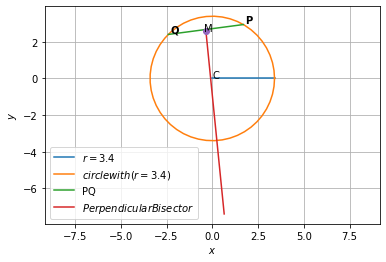
\includegraphics[width=\columnwidth]{FIG.3.png}
    \caption{perpendicular bisector of the chord passes through the center}
    \label{fig: perpenicular bisector of the chord passes through the center}
\end{figure}






\end{document}



\end{document}



\end{document}
